\documentclass[12pt,a4paper]{article}
\usepackage[utf8]{inputenc}
\usepackage[shortlabels]{enumitem}
\usepackage{fontawesome}
%Set page layout parameters
\usepackage[
top=4cm,
bottom=2cm,
left=2cm,
right=2cm,
headheight=2cm,
footskip=1cm,
marginparwidth=2cm]{geometry}
\usepackage{amsmath}
\usepackage{cancel}
\usepackage{hyperref}
\usepackage[dvipsnames]{xcolor}
\usepackage{multicol}
% To use color boxes
\usepackage{tcolorbox}
\usepackage{lipsum}
\tcbuselibrary{listings,theorems,skins,vignette,raster,breakable,magazine,poster,fitting,hooks}
\newcounter{ejemplo}
%Images path
\graphicspath{{images/}}
\usepackage{float} %provide us with the option H
\usepackage{fancyhdr}
\usepackage{tikz}
\usepackage{tikzpagenodes}
%to redefine figure caption 
\renewcommand{\figurename}{Figura}
%change text font
\usepackage[T1]{fontenc}
\usepackage{tgtermes} % LaTeX will use the TEX Gyre Bonum font family 


\urlstyle{same}
\usepackage{vwcol}
\definecolor{subtitle_yellow}{RGB}{252,213,129}
\definecolor{title_yellow}{RGB}{249,175,16}
\definecolor{steel_blue_title}{RGB}{93,138,168}
\definecolor{pewter_blue_subtitle}{RGB}{149,178,198}
\definecolor{ecru_circle}{RGB}{215,190,130}
\definecolor{ecru_circle1}{RGB}{68,148,173}

\newcommand{\myfirststyle}{%
	\begin{tikzpicture}[remember picture, overlay]
		
		%top border
		\fill[fill=steel_blue_title](current page.north west) rectangle ([yshift=-15mm]current page.north east);
		
		\fill[fill=pewter_blue_subtitle]([yshift=-17mm]current page.north west) rectangle ([yshift=-30mm]current page.north east);
		
		%page box
		%\draw[lightgray, fill=Rhodamine, fill opacity=0.05, line width=1mm, rounded corners=3mm] ([xshift=-5mm,yshift=5mm]current page text area.north west) rectangle ([xshift=5mm,yshift=-5mm]current page text area.south east);
		
		%bottom box
		\fill[fill=pewter_blue_subtitle](current page.south west) rectangle ([yshift=10mm]current page.south east);
		
		%page circle
		\draw[white,fill=ecru_circle1,line width=2mm] ([xshift=-5mm,yshift=25mm]current page text area.north east) circle (1); 
		
		
		%page number text        
		%\node[anchor=center] at ([xshift=-5mm,yshift=25mm]current page text area.north east) {\Huge\bfseries\sffamily\color{white}{\thepage}};
		
		%title text
		\node[anchor=west] at ([yshift=32mm]current page text area.north west) {\Huge\bfseries\sffamily\color{white}{Ley de Ohm en circuitos resistivos}};
		
		%subtitle text
		\node[anchor=west] at ([xshift=10mm,yshift=16mm]current page text area.north west) {\Large\bfseries\sffamily\color{white}{}};
		
		%footer text
		\node[anchor=center] at ([yshift=-15mm]current page text area.south) {\large\bfseries\sffamily\color{white}{Created by: Belmont Dubois}};
		
	\end{tikzpicture}
}


%create page style
\fancypagestyle{MyFirstStyle}{%
	\fancyhf{}
	\fancyhead[C]{\myfirststyle}
	\renewcommand{\headrulewidth}{0pt}
}%

\pagestyle{MyFirstStyle}

\colorlet{colexam}{red!75!black}
\newtcolorbox[use counter=ejemplo]{myexample}{%
	empty,title={Ejemplo \thetcbcounter},attach boxed title to top left,
	boxed title style={empty,size=minimal,toprule=2pt,top=4pt,
		overlay={\draw[colexam,line width=2pt]
			([yshift=-1pt]frame.north west)--([yshift=-1pt]frame.north east);}},
	coltitle=colexam,fonttitle=\Large\bfseries,
	before=\par\medskip\noindent,parbox=false,boxsep=0pt,left=0pt,right=3mm,top=4pt,
	breakable,pad at break*=0mm,vfill before first,
	overlay unbroken={\draw[colexam,line width=1pt]
		([yshift=-1pt]title.north east)--([xshift=-0.5pt,yshift=-1pt]title.north-|frame.east)
		--([xshift=-0.5pt]frame.south east)--(frame.south west); },
	overlay first={\draw[colexam,line width=1pt]
		([yshift=-1pt]title.north east)--([xshift=-0.5pt,yshift=-1pt]title.north-|frame.east)
		--([xshift=-0.5pt]frame.south east); },
	overlay middle={\draw[colexam,line width=1pt] ([xshift=-0.5pt]frame.north east)
		--([xshift=-0.5pt]frame.south east); },
	overlay last={\draw[colexam,line width=1pt] ([xshift=-0.5pt]frame.north east)
		--([xshift=-0.5pt]frame.south east)--(frame.south west);},%
}

\DeclareTotalTCBox{\commandbox}{ s v }
{verbatim,colupper=pink,colback=black!75!white,colframe=black}
{\IfBooleanT{#1}{\textcolor{cyan}{\ttfamily\bfseries SELECT }}%
	\lstinline[language=command.com,keywordstyle=\color{blue!35!white}\bfseries]^#2^}

\DeclareTotalTCBox{\commandboxa}{ s v }
{verbatim,colupper=white,colback=gray!75!white,colframe=gray}
{\IfBooleanT{#1}{\textcolor{cyan}{\ttfamily\bfseries SELECT }}%
	\lstinline[language=command.com,keywordstyle=\color{blue!35!white}\bfseries]^#2^}

\begin{document}
	
	En un circuito mixto se combinan las características de un circuito en serie y un circuito en paralelo. Por lo tanto, algunas cargas están conectadas en serie para que por ellas circule la misma corriente, mientras que otras lo están en paralelo para que tengan el mismo voltaje, es decir:

	\begin{tcolorbox}[colback=red!10!white,colframe=red!50!black,title=\faWarning \,Enunciado 1: Corriente en un circuito en serie]
		\textbf{La corriente a través de los elementos de un circuito en serie siempre es la misma}
	\end{tcolorbox}

	\begin{tcolorbox}[colback=red!10!white,colframe=red!50!black,title=\faWarning \,Enunciado 2: Voltaje a través de un circuito en paralelo]
		\textbf{El voltaje a través de los elementos conectados en paralelo siempre es el mismo}
	\end{tcolorbox}

	Dado cualquier circuito resistivo mixto (funcionando también con impedancias $Z=R+jX$), el primer paso es reducir dicho circuito hasta su mínima expresión hasta obtener una sola resistencia equivalente o total ($R_T$ o $R_{eq}$) esto con el fin de obtener la corriente total que circula por el circuito.\\
	
	Por ejemplo, sea el circuito de la figura 1(a), lo reducimos hasta llegar a la resistencia total $R_T = 50 \Omega$. Tenga muy en cuenta cómo se llegaron a obtener las resistencias $R_7$, $R_8$, $R_9$ y $R_T$. 
	\begin{figure}[H]
		\centering
		
\includegraphics[width=\textwidth]{circuito}
		\caption{}
		\label{fig:circuito}
	\end{figure}

	\newpage
	
	Una vez obtenida la resistencia total procedemos a calcular la corriente total mediante el uso de la ley de Ohm
	\begin{tcolorbox}[colback=red!5!white,colframe=red!75!black,width=(\linewidth+0.45cm)]
		\begin{equation}
			I_T = \frac{V_T}{R_T} = \frac{100V}{50\Omega} = 2 A\nonumber
		\end{equation}
	\end{tcolorbox}

	Ya hemos conseguido la corriente total, pero, ¿cómo obtenemos el voltaje y las corrientes a través de las demás resistencias del circuito? Simple, analizando el circuito de la figura 1 en sentido inverso y teniendo presentes los Enunciados 1 y 2
	
	Es decir, de acuerdo a la figura 1(e) sabemos que 
	\begin{align}
		R_T = R_1 + R_2 + R_9\nonumber
	\end{align}
	Es decir, $R_T$ se calculó debido a la combinación en \textbf{serie} de $R_1$, $R_2$ y $R_9$. Por tanto, de acuerdo al Enunciado 1, la corriente a través de los elementos conectados en serie es la misma, así:
	
	\begin{tcolorbox}[colback=red!5!white,colframe=red!75!black,width=(\linewidth+0.45cm)]
		\begin{equation}
			I_T = I_{R_1} = I_{R_2} = I_{R_9} = 2A\nonumber
		\end{equation}
	\end{tcolorbox}

	Ahora empleamos la ley de Ohm para encontrar los voltajes en esas tres resistencias:
	\begin{align}
		V_{R_1} &= R_1 I_{R_1} = (14\Omega)(2A) = 28V\nonumber\\
		V_{R_2} &= R_2 I_{R_2} = (30\Omega)(2A) = 60V\nonumber\\
		V_{R_9} &= R_9 I_{R_9} = (6\Omega)(2A) = 12V\nonumber
	\end{align}
	Con esto, ya tenemos los valores de voltaje y corriente de las resistencias de la figura 1(d). De esta misma figura sabemos que 
	\begin{align}
		R_9 = R_5 || R_8\nonumber
	\end{align}
	Es decir, que $R_9$ se obtuvo debido a la combinación en \textbf{paralelo} de $R_5$ y $R_8$. Ya que dichas resistencias están en paralelo empleamos el Enunciado 2 la cual indica que el voltaje a través de los elementos conectados en paralelo siempre será el mismo. Con esto en mente sabemos que 
	
	\begin{tcolorbox}[colback=red!5!white,colframe=red!75!black,width=(\linewidth+0.45cm)]
		\begin{equation}
			V_{R_9} = V_{R_5} = V_{R_8} = 12V
		\end{equation}
	\end{tcolorbox}
	Ahora nos queda calcular las corrientes en $R_5$ y $R_8$
	\begin{align}
		I_{R_5} = \frac{V_{R_5}}{R_5} = \frac{12V}{10\Omega} = 1.2A\nonumber\\
		I_{R_8} = \frac{V_{R_8}}{R_8} = \frac{12V}{15\Omega} = 0.8A\nonumber
	\end{align}

	Con esto ya sabemos cuales son los voltajes y corrientes a través de los elementos del circuito de la figura 1(c). De esta misma figura sabemos que
	\begin{align}
		R_8 = R_6 + R_7\nonumber
	\end{align}
	Es decir, que $R_8$ se obtuvo mediante la combinación en \textbf{serie} de $R_6$ y $R_7$. Esto nos devuelve al enunciado 1, por lo que fácilmente deducimos que:
	\begin{tcolorbox}[colback=red!5!white,colframe=red!75!black,width=(\linewidth+0.45cm)]
		\begin{equation}
			I_{R_8} = I_{R_6} = I_{R_7} = 0.8A\nonumber
		\end{equation}
	\end{tcolorbox}

	Ahora calculamos los voltajes en $R_6$ y $R_7$
	\begin{align}
		V_{R_6} &= R_6 I_{R_6} = (7\Omega)(0.8A) = 5.6V\nonumber\\
		V_{R_7} &= R_7 I_{R_7} = (8\Omega)(0.8A) = 6.4V\nonumber
	\end{align}

	Con esto ya sabemos los voltajes y corrientes de los elementos del circuito de la figura 1(b). De esta misma figura observamos que
	\begin{align}
		R_7 = R_3 || R_4\nonumber
	\end{align}

	Es decir, que $R_7$ se obtuvo de la combinación en \textbf{paralelo} de $R_3$ y $R_4$, por lo tanto
	\begin{tcolorbox}[colback=red!5!white,colframe=red!75!black,width=(\linewidth+0.45cm)]
		\begin{equation}
			V_{R_7} = V_{R_3} = V_{R_4} = 6.4V\nonumber
		\end{equation}
	\end{tcolorbox} 
	Y calculamos las corrientes:
	\begin{align}
		I_{R_3} = \frac{V_{R_3}}{R_3} = \frac{6.4V}{12\Omega} = 533.33 mA\nonumber\\
		I_{R_4} = \frac{V_{R_4}}{R_4} = \frac{6.4V}{24\Omega} = 266.66 mA\nonumber
	\end{align}
	\begin{figure}[H]
		\centering
		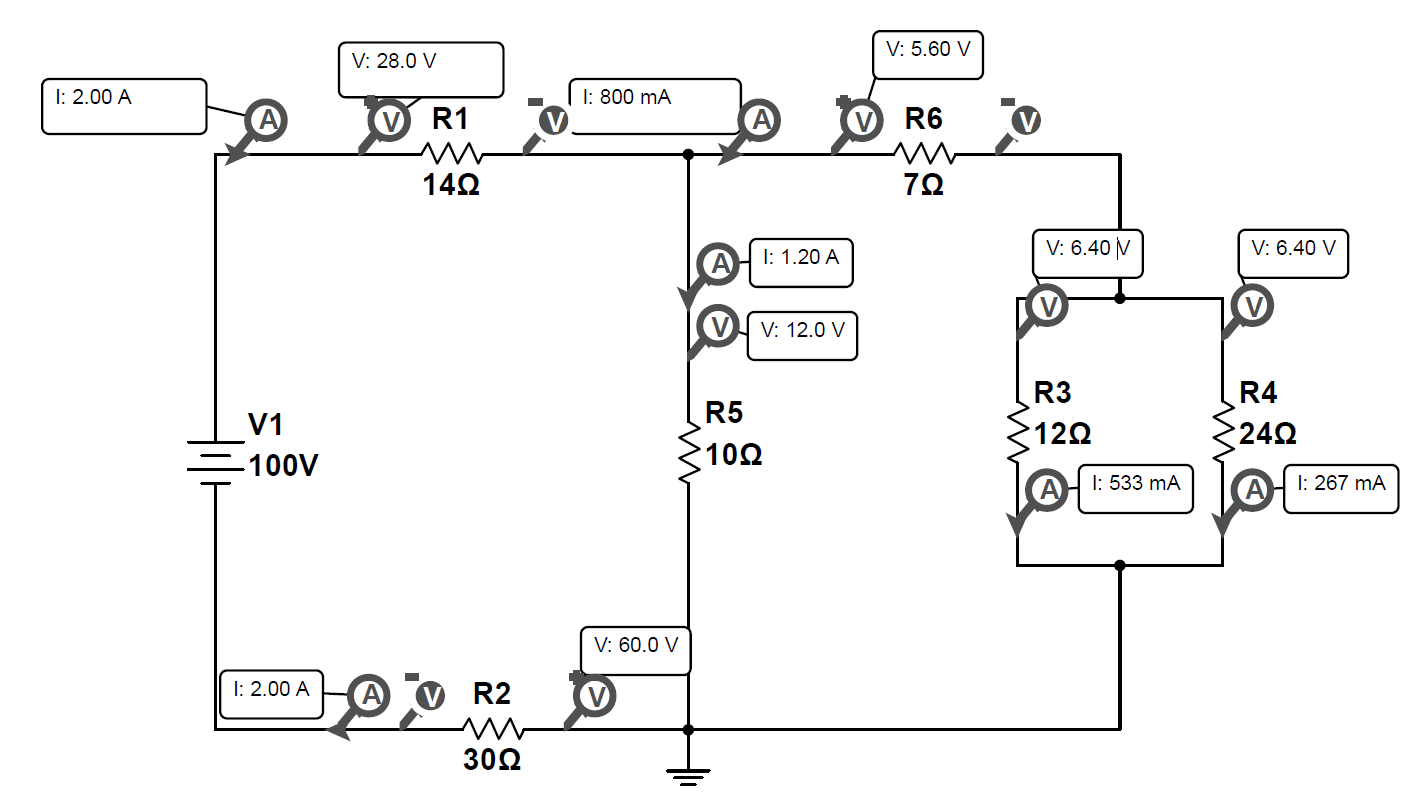
\includegraphics[width=\textwidth]{circuito1}
		\caption{}
		\label{fig:circuito1}
	\end{figure}

	\begin{myexample}
		Calcula los voltajes y corrientes en el circuito de la figura 3
		\begin{figure}[H]
			\centering
			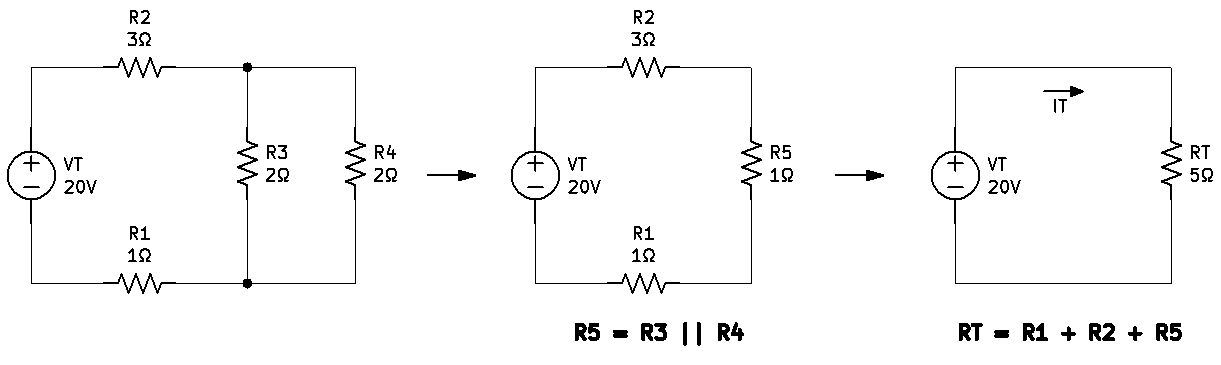
\includegraphics[width=\textwidth]{circuito2}
			\caption{}
			\label{fig:circuito2}
		\end{figure}
	\end{myexample}
\end{document} 

